\documentclass[a4paper,12pt]{report}
%\usepackage{algorithmic}
%\usepackage[linesnumbered,ruled,vlined]{algorithm2e}
\usepackage[margin=2cm]{geometry}
\usepackage[utf8]{inputenc}
\usepackage{listings} 
\usepackage{graphicx} 
\usepackage{color}
\usepackage{xcolor}
\usepackage{hyperref}
%\usepackage{mdframed}

\newcommand{\currentdata}{ 1 February 2017}
\newtheorem{example}{Example}

\begin{document}
\vspace{-5cm}
\begin{center}
Departamentul de Calculatoare \c si Tehnologia Informa\c tiei\\
Universitatea Tehnic\u a din Cluj-Napoca\\

\includegraphics[width=10cm]{fig/footer}
\end{center}
\vspace{1cm}
%\maketitle
\begin{center}
  \begin{Large}
    \textbf{Sisteme Inteligente}\\
  \end{Large}
  
  \textit{Activitate de laborator 2016-2017}\\
  \vspace{3cm}
  Titlul proiectului: Clasificarea email-urilor\\
  Tool: LibSVM\\
  \vspace{1.5cm}
  Nume: B\'anhidi Zolt\'an\\
  Grupa: 30234\\
  Email: banhidizoli@gmail.com\\
  
  \vspace{6cm}
  Prof. dr. ing. Adrian Groza\\
  Adrian.Groza@cs.utcluj.ro\\
  
  \vspace{1cm}
  
\includegraphics[width=10cm]{fig/footer}
\end{center}

\tableofcontents







\chapter{Instalarea programelor ($W_2$)}

  \par
  \^In cadrul acestui proiect este folosit programul \textit{LibSVM} pentru clasificarea email-urilor. Pentru rularea
  proiectului este necesar\u a instalarea ma\c sinii virtuale Java, deoarece prelucrarea \c si transformarea datelor
  \^in formatul numeric \^in\c teles de \textit{LibSVM} este realizat\u a de un program scris \^in limbajul Java.
  
  \^In continuare se prezint\u a metoda de instalare a tool-ului \textit{LibSVM} \c si a pachetului Oracle JDK
  (\textit{Java Development Kit})
  pentru sistemul de operare Ubuntu 16.10 64, versiunea pe 64 de bi\c ti (Oracle JDK este preferat fa\c t\u a de 
  versiunile Open JDK pentru perfoman\c t\u a \c si compatibilitate maxim\u a).
  
  \par
  Programul \textit{LibSVM} se poate desc\u arca de la adresa 
  \href{https://www.csie.ntu.edu.tw/~cjlin/libsvm/}{https://www.csie.ntu.edu.tw/~cjlin/libsvm/}.
  Dup\u a finalizarea desc\u arc\u arii, fi\c sierul desc\u arcat poate fi dezarhivat folosind comanda
  \begin{center}
    \verb|tar -xvzf nume_fisier|
  \end{center}

  \par
  Dup\u a dezarhivare, trebuie s\u a navig\u am \^in interiorul fi\c sierului dezarhivat cu comanda linux 
  \verb|cd nume_fisier_dezarhivat|. Pentru a compila programul, trebuie doar s\u a introducem comanda 
  \verb|make|. Dup\u a executarea 
  compil\u arii vor fi generate urm\u atorele executabile:
  
  \begin{center}
    \begin{tabular}{ | l | p{8cm} | }
      \hline
      \textbf{Nume fi\c sier executabil} & \textbf{Descriere} \\
      \hline
      
      \verb|svm-scale| & Programul care scaleaz\u a datele de intrare pentru a asigura acurate\c te c\^at mai mare \\
      \hline
      
      \verb|svm-train| & Programul care generaez\u a un model pe baza exemplelor furnizate (\^inva\c t\u a) \\
      \hline
      
      \verb|svm-predict| & Programul cu ajutorul c\u areia putem rula testele pe baza 
	modelului generat prin \^inv\u a\c tare \\
      \hline      
    \end{tabular}
  \end{center}

  \par
  \^In continuare se prezint\u a instalarea pachetului \textit{Java Development Kit}. Acest pachet con\c tine at\^at 
  ma\c sina virtual\u a Java c\^at \c si compilatorul Java respectiv biblioteca standard a limbajului.
  JDK poate fi desc\u arcat de pe pagina web 
  
  \begin{center}
    \href{http://www.oracle.com/technetwork/java/javase/downloads/jdk8-downloads-2133151.html}
    {http://www.oracle.com/technetwork/java/javase/downloads/jdk8-downloads-2133151.html}
  \end{center}
  
  Trebuie selectat\u a versiunea destinat\u a pentru sistemul de operare Linux pe 64 de bi\c ti (
  \textit{x64}) cu extensia \textit{tar.gz}. Dup\u a finalizarea desc\u arc\u arii fi\c sierului, 
  acesta trebuie dezarhivat cu ajutorul comenzii de dezarhivare 
  folosite \c si la \textit{LibSVM}. Fi\c sierul dezarhivat trebuie copiat \^in directorul 
  \verb|/usr/lib/jvm| cu ajutorul comenzii:
  
  \begin{center}
    \verb|mv nume_fisier /usr/lib/jvm|
  \end{center}
  
  \par
  Urm\u atorul pas este s\u a configur\u am ma\c sina virtual\u a Java instalat\u a \^in acest mod
  ca \c si cel de baz\u a al sistemului.
  Prima dat\u a trebuie s\u a comunic\u am sistemului de operare instalarea cu ajutorul comenzilor
  
  \begin{center}
    \begin{verbatim}
	sudo update-alternatives --install 
	  /usr/bin/java java /usr/lib/jvm/nume_fisier/jre/bin/java 2000
    \end{verbatim}

    \begin{verbatim}
	sudo update-alternatives --install 
	  /usr/bin/javac javac /usr/lib/jvm/nume_fisier/bin/javac 2000
    \end{verbatim}
  \end{center}
  
  \par
  Apoi trebuie s\u a configur\u am acestea. Trebuie selectat \^in fiecare caz componenta nou instalat\u a 
  \^in listele afi\c sate dup\u a rularea comenzilor
  
  \begin{center}
    \begin{verbatim}
      sudo update-alternatives --configure java
      sudo update-alternatives --configure javac
    \end{verbatim}
  \end{center}
  
  

  
  
  
  



\chapter{Rularea \c si \^in\c telegerea exemplelor ($W_3$)}

  \par
  Support Vector Machines (SVM) este o tehnic\u a des folosit\u a \^in domeniul inteligen\c tei artificiale
  pentru clasificarea datelor. SVM este de fapt o colec\c tie de algoritmi de \^inv\u a\c tare
  (machine learning) care sunt folosite pentru clasificarea datelor.
  
  \par
  O particularitate a SVM-ului este c\u a algoritmii pot prelucra doar date numerice. Astfel \^in cazul \^in care
  se dore\c ste clasificarea unei date de alt tip (de exemplu text), acesta trebuie 
  transformat \^intr-o reprezentare numeric\u a.
  
  \par
  \^In cadrul acestui proiect va fi folosit programul \textit{LibSVM} pentru clasificarea email-urilor. 
  Acesta este o implementare r\u asp\^andit\u a a SVM.
  Deoarece proiectul se concentreaz\u a pe clasificarea texturilor folosind algoritmii SVM, \^in clasificare se vor
  lua \^in considerare dor subiectele email-urilor. Aceste \c siruri de caractere sunt prelucrate \c si transformate
  de c\u atre un program Java \^in format numeric \c tin\^and cont de caracterisiticile semnificative ale \c sirurilor de 
  caractere. Valorile ob\c tinute trebuie scalate folosind \verb+svm-scale+
  pentru a asigura o acurate\c te c\^ at mai mare a rezultatelor. Scalarea const\u a din aplicarea unei func\c tii 
  de transformare liniar\u a
  a numerelor din intervalul $[a,b]$ \^in intervalul $[0,1]$ sau $[-1,1]$ ob\c tinute prin 
  convertirea \c sirurilor de caractere.
  
  \par 
  Datele ob\c tinute dup\u a scalare sunt folosite pentru a antrena re\c teaua SVM (\^inv\u a\c tare), 
  care dup\u a aceast\u a 
  etap\u a gener\^and un a\c sa numit \textit{model} este capabil s\u a clasifice noile date de intrare. Este important ca datele de
  intrare s\u a fie generale, con\c tin\^and c\^at mai multe exemple din fiecare clas\u a (clasele sunt acele tipuri \^in 
  care SVM trebuie s\u a clasifice \c sirurile de caractere prelucrate).
  
  \par
  Datele de antrenare ale \textit{LibSVM} au urm\u atorul format:
  
  \begin{verbatim}
    label index1:value1 index2:value2 ...
  \end{verbatim}
  
  \verb|label| este un num\u ar \^intreg care indic\u a num\u arul clasei de care apar\c tine data respectiv\u a.
  \verb|indexi| sunt valori \^intregi \^in ordine cresc\u atoare care reprezint\u a num\u arul caracteristicii, iar 
  \verb|valuei| este num\u arul real care indic\u a caracteristica respectiv\u a a datei curente. Altfel spus 
  data curent\u a are valoarea \verb|valuei| la caracteristica \verb|indexi|.
  
  \par
  Datele de intrare \c si de test au formatul prezentat, \c si sunt separate printre ele prin caracterul 
  \verb|'\n'|. Deci fiecare dat\u a trebuie s\u a fie conform formatului prezentat \c si s\u a fie
  amplasat\u a pe un r\^and al fi\c sierului de intrare pentru \^inv\u a\c tare. Nu este permis\u a amplasarea
  mai multor date pe acela\c si r\^and.

  \par
  Un exemplu u\c sor de \^in\c teles este cel \^in care dorim s\u a clasific\u am propozi\c tiile din punctul de vedere al 
  complexit\u a\c tii acestora. Avem deci propozi\c tii simple \c si compuse. Lu\u am \^in considerare de
  exemplu caracteristici precum:
   
  \begin{itemize}
     \item{} num\u arul virgulelor din propozi\c tie
     \item num\u arul total al caracterelor
     \item num\u arul de apari\c tii al cuvintelor de leg\u atur\u a (de exemplu: 
      \textit{\c si}, \textit{respectiv}, \textit{a\c sadar}, \textit{totodat\u a} etc.)
  \end{itemize}
  
  \par
  Num\u arul virgulelor va apare la indexul 1, num\u arul caracterelor la indexul 2 \c si num\u arul 
  de cuvinte de leg\u atur\u a la indexul 3. Consider\u am c\u a propozi\c tia simpl\u a are eticheta clasei 
  -1 \c si cea compus\u a eticheta clasei 1. 
  
  \par
  Astfel propozi\c tia \textit{R\u azvan merge la \c scoal\u a.} este reprezentat\u a prin linia
  
  \begin{verbatim}
    -1 1:0 2:23 3:0
  \end{verbatim}

  Identic propozi\c tia \textit{Anca este harnic\u a, a\c sadar ea \^inva\c t\u a \^in fiecare zi.} este
  reprezentat\u a prin linia
  
  \begin{verbatim}
    1 1:1 2:50 3:1
  \end{verbatim}
  
  Dup\u a crearea fi\c sierului de antrenare (denumit \verb|input.txt| care con\c tine 
  date precum cele dou\u a enumerate mai sus), se antreneaz\u a SVM-ul care va rezulta 
  un fi\c sier denumit \verb+model+ folosind comanda
  
  \begin{center}
    \verb|./svm-train input.txt model|
  \end{center}
  
  \par
  Apoi se creeaz\u a fi\c sierul de test (\verb+test.txt+ care are 
  aceea\c si forma ca \c si fi\c sierul \verb|input.txt|).
  Apel\^and predic\c tia pe acest fi\c sier \textit{LibSVM} va determina de care clas\u a (-1 sau 1)
  apar\c tine fiecare propozi\c tie \c si apoi va compara rezultele ob\c tinute cu cele date (autoevaluare). Astfel se 
  calculeaz\u a acurate\c tea. Predic\c tia se ruleaz\u a folosind comanda
  
  \begin{center}
    \verb|./svm-predict test.txt model output.txt|
  \end{center}

  \par
  Fi\c sierul text generat \verb+output.txt+ con\c tine pe fiecare linie num\u arul clasei de care apar\c tine 
  propozi\c tia codificat\u a prin caracteristici de pe aceea\c si linie din fi\c sierul
  \verb+test.txt+ conform SVM-ului.
  
  
  
  
  

 
 
\chapter{Understanding conceptual instrumentation ($W_4$)}
\label{ch:tool}


The teaching objectives for this week are:
\begin{enumerate}
 \item To understand the algorithm(s) on which your tool relies.
\item To get used with writing algorithms in Latex
\end{enumerate}

Latex provides various environments for writing algorihms, including: 
\texttt{algorithm, algorithmic, algorithmicx, algpseudocode, algorithm2e}.

The following example algorithm has been taken from~\cite{7034697}.


\section{Exercises}
\begin{enumerate}
 \item Big O complexity
 \item Which are the latex options to write algorithms? 
 Describe in one paragraph the main features of one such package for algorithms.
\end{enumerate}

\fbox{\begin{minipage}{16cm}
Solution to exercise 1       
\end{minipage}}
\vspace{0.5cm}

\fbox{\begin{minipage}{16cm}
Solution to exercise 2       
\end{minipage}}
\vspace{0.5cm}









\chapter{Descrierea proiectului ($W_5$)}

  \par
  Proiectul de fa\c t\u a are titlul \textit{Clasificarea email-urilor}. A\c sa cum sugereaz\u a \c si titlul
  scopul aplica\c tiei dezvoltate este filtrarea \c si clasificarea email-urilor. Se consider\u a urm\u atoarele
  dou\u a clase de email-uri:
  
  \begin{itemize}
    \item email-uri cu caracter de reclam\u a (advertising email)
    \item alte email-uri
  \end{itemize}

  Email-urile trebuie prelucrate automat de c\u atre program. Pentru aceasta se dezvolt\u a o aplica\c tie Java 
  care folose\c ste biblioteca \textit{JavaMail}. Acesta se conecteaz\u a la contul de email al utilizatorului folosind 
  conexiunea internet \c si descarc\u a subiectele umail-urilor necitite.
  
  \par
  Programul Java pe l\^ang\u a desc\u arcarea email-urilor care trebuie analizate mai are o component\u a. Aceasta
  transform\u a \c sirurile de caractere (subiectele fiec\u arui email) \^intr-o reprezentare numeric\u a \^in\c teleas\u a
  de \textit{LibSVM}. \^In aceast\u a transformare trebuie s\u a se \c tin\u a cont de caracteristicile relevante ale 
  \c sirului de caractere \^in privin\c ta clasific\u arii \^in cele dou\u a categorii. De exemplu cuvintele precum 
  \textit{pre\c t, reducere} sau \textit{ofert\u a} mai mult ca sigur apar\c tin unei reclame.
  
  \par
  Re\c teaua SVM este antrenat\u a cu ajutorul email-urilor personale recep\c tionate de-a lungul timpului. Setul de date
  trebuie s\u a cuprind\u a cca. jum\u atate de email-uri reclam\u a \c si cealalt\u a jum\u atate alte email-uri. Acestea
  vor fi convertite automat folosind programul scris \^in Java dar necesit\u a \c si interven\c tie 
  umana pentru a le clasifica.
  
  \par
  Pe baza cuno\c stin\c telor asimilate prin \^inv\u a\c tare SVM va putea decide dac\u a un email nou este sau nu
  o reclam\u a. Pentru a \^imbun\u ata\c ti acurate\c tea programului (rata de clasificare corect\u a), \^inainte de
  etapa de \^inv\u a\c tare, caracteristicile trebuie scalate (din intervalul de care apar\c tin acestea se vor transforma
  printr-o func\c tie liniar\u a \^in intervalul $[0,1]$).
  
  \par
  Scopul aplica\c tiei este deci clasificarea email-urilor \^in cele dou\u a categorii amintite. Aceast\u a opera\c tie
  poate fi efectuat\u a cu ajutorul antrenamentului prin email-urile personale primite de-a lungul timpului de la 
  diferite market-uri online (de exemplu \textit{emag.ro, cel.ro, flanco.ro}) \c si alte email-uri care apar\c tin 
  clasei secunde.
  
  \par
  Datele de intrare ale aplica\c tiei sunt:
  
  \begin{itemize}
    \item adres\u a de email
    \item parola contului
  \end{itemize}
  
  Datele de ie\c sire sunt dou\u a liste de email-uri: o list\u a care con\c tine emailurile necitite reclam\u a \c si 
  cealalt\u a list\u a populat\u a cu email-urile care nu sunt reclame.
  
  \par
  Diagrama bloc al alica\c tiei dezvoltate este reprezentat\u a \^in figura \ref{fig.blocDiagram}.
  
  \begin{figure}[h]
    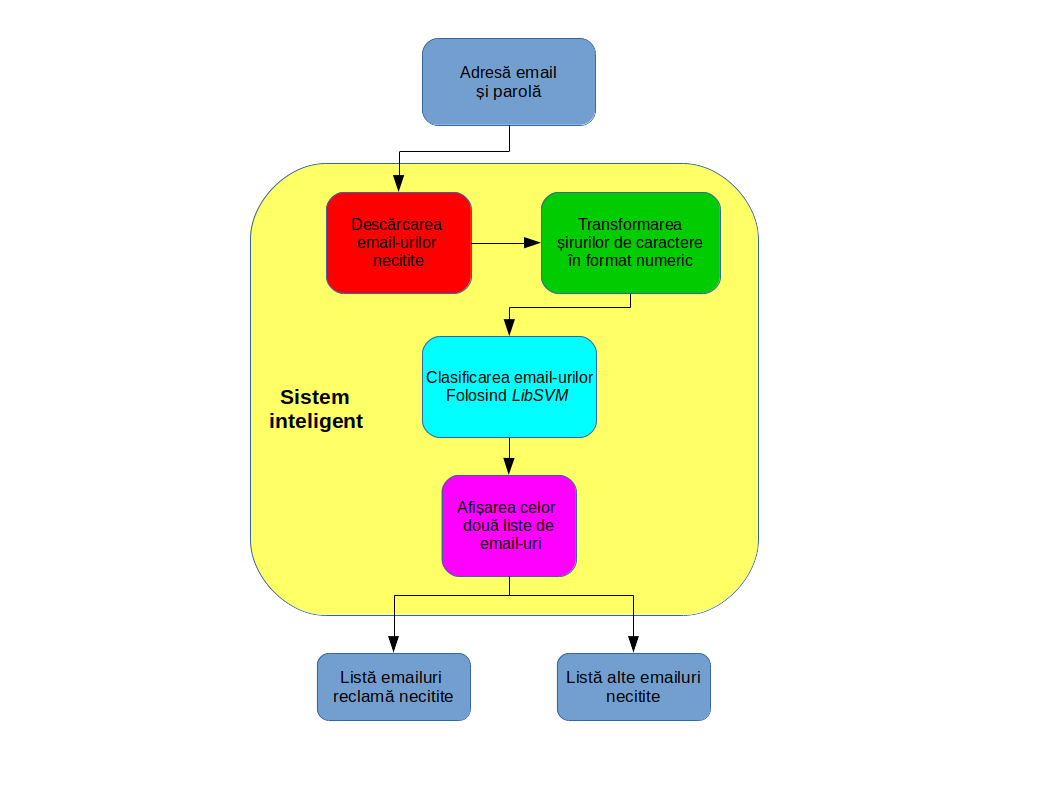
\includegraphics[scale=0.7]{fig/BlocDiagram.png}
    \caption{Diagrama bloc a aplica\c tiei}
    \label{fig.blocDiagram}
  \end{figure}
  


  
  
  



\chapter{Preliminary results ($W_7$)}
This section corresponds to the midway report in week 7.
The teaching objectives for this week are:
\begin{enumerate}
 \item To prove that you have managed to write few lines of code of your own.
\item To prove that the knowledge or data required are already obtained.
\end{enumerate}

These objectives decreases the risk to fail. 
You should be aware that failing to meet the above objectives in week 
7 indicates high risks in obtaining relevant results at the end of the semester.
Take urgent measures to overcome these difficulties.


\section{Exercises}
\begin{enumerate}
\item Write the preliminary results explaining any realizations or insights found during the research of the subject.
\item Discuss new information and questions found during the domain investigation or during coding.
\end{enumerate}








\chapter{Implementation details ($W_9$)}

The teaching objectives for this week are:
\begin{enumerate}
 \item Illustrate each aspect of the reality that you have 
 modelled in your solution.
\item To explain the relevant code from your scenario.
\end{enumerate}

\vspace{0.5cm}

My personal objectives for this class are:
\begin{enumerate}
 \item 
 \item 
\end{enumerate}

Projects in artificial intelligence consist of developing new solutions. 


\section{Relevant code}

Provide the relevant code (see an example in Fig.~\ref{fig:code}).
You can use "verbatim" package or "listing" package. 
Complement the code with its corresponding textual description.

\begin{figure}
\begin{verbatim}
(full-reset)
(instance a Argument)
(related a b attacks)
(concept-instances Argument) 
\end{verbatim}
\caption{Modelling arguments in Racer.}
\label{fig:code} 
\end{figure}

The eager student may use concepts from \textit{literate programming}.

\section{Common bad practice in AI undergraduate projects}

\paragraph{The over-estimated AI programmer.} $ $

{\it Bad practice}: Excepting few genial students, you tend to overestimate your AI-programming abilities. 
That is, you start to write a large amount of code. (Here large might be 20 lines).
When testing it, nothing run. 
You start to debug a line or to remove it.
Your program will not run this time too. 
You remove or comment another line. 
And so on, until you have a single line of code.
If you are lucky, that could run. 
But you lose a lot of time in this enterprise.

{\it Solution}: In the early stage of writing code, write a line of code and test it. 
If it works, write another line and test it. 
And so on. 
That is, you are exploiting the interactive environments provided by 
AI tools or languages like LISP and PROLOG.
You should hold your horses and 
have the most possible skeptical attitude towards your code.  
As you get experience, your will be noticing that writing 
AI-declarative code is more effective than procedural one.  


\paragraph{The eyewash bug.} $ $
{\it Bad practice}: You spend most of your programming time to develop a GUI for your AI-system. 
Don't bother. I am sympathetic with Sania Twain's view on GUIs: "You don't impress me much".
Such things are indeed important in computer science, but not relevant in this AI class.


%\paragraph{The stucker bug} 

\paragraph{The not-organised student.}
You are not organised, if something like this will happen to you:
\begin{itemize}
 \item You do not find your project and yield "Someone removed my project!". 
Most of the time your are logged with a different user as usual. 
Check this with \texttt{who am i}. 
This is not a rhetorical question, but a Linux command.
\item You are working in a different directory. 
Type \texttt{pwd} and \texttt{ls} to check that your executables are indeed in the current working directory.
If you have been lazy to set your PATH variable, you might just forgot to type \texttt{./} 
for executing the command in the current directory.
\end{itemize}

\paragraph{The omniscient student.}
You are in this cathegory if you fail to add references. 
Reading relevant references is mandatory to deliver a decent project. 

\section{Exercises}
\begin{enumerate}
 \item What latex packages can be used to format code? 
 \item 
\end{enumerate}

\fbox{\begin{minipage}{16cm}
Solution to exercise 1       
\end{minipage}}
\vspace{0.5cm}

\fbox{\begin{minipage}{16cm}
Solution to exercise 2       
\end{minipage}}
\vspace{0.5cm}




\chapter{Tool expressivity ($W_{10}$)}


The teaching objectives for this week are:
\begin{enumerate}
 \item Describe each technical instrumentation provided 
by the tool that was enacted in your implementation.
\end{enumerate}

\vspace{0.5cm}

My personal objectives for this class are:
\begin{enumerate}
 \item 
 \item 
\end{enumerate}



%For instance:
%{\it "Racer offers also the capability to use {\it rules}. 
%he code in Fig.~\ref{fig:rules} illustrates my rule used to create instances of type student."}


\chapter{Graphs and experiments ($W_{11}$)}

The objectives for this week are:
\begin{enumerate}
 \item To describe and interpret each experiment that you have performed
\end{enumerate}

\vspace{0.5cm}

My personal objectives for this class are:
\begin{enumerate}
 \item 
 \item 
\end{enumerate}


An experiment investigates how some variables are related. 
Usually, experiments verify a previosly formulated hypothesis.
Such hypothesis may investigate how your software degrades its performance with larger inputs.
You will need to run simulations to see how your implementation is affected by different inputs.


Note that running experiments mean more than testing your solution. 
It helps to describe and prove how did you test your implementation.
Moreover, during this lab, you will often need to: 
1) generate random data for your algorithms,
2) measure their performance (number of operations, execution time),
3) draw charts,
4) interpret the obtained results.

The eager student might want to take a look at literature on how to design computer experiments, such as~\cite{fang2005design}. Section 5.6 from~\cite{fang2005design} might be of particular interest for some of you. 
If your experiments include a stochastic parameter, you need to include a test for statistical significance. 
This is important to prove that your ouputs are not a random effect.



\begin{figure}
%\includegraphics[width=8cm]{} 
Graphs always impress teachers...
\caption{Increasing the accuracy with the number of samples.}
\label{fig:accuracy}
\end{figure}

You should develop a test suite that can be used to show your code works correctly under a various conditions/problems/scenarious.


\section{Evaluation metrics}



\chapter{Related work and documentation ($W_{12}$)}

The teaching objectives for this week are:
\begin{enumerate}
 \item To compare your results to related work.
\item To discuss the advantages and limitations of your solution.
\item To deliver a professional documentation of your work.
\end{enumerate}

\vspace{0.5cm}

My personal objectives for this class are:
\begin{enumerate}
 \item 
 \item 
\end{enumerate}


This chapter convinces me that you know how your work fits into the larger domain area.


%For instance: \cite{chesnevar:Survey2000}

\section{Related approaches}
You need to support your opinions with trustworthy evidence and references.
You need also to decide how your problem fits into a wider context.
The quality of your reference is a strong indicator that you 
managed to scrutinise different perspectives on the topic.
Proving understanding of the references is the foundation of a good grade. 
By start coding without reading relevant references, you will most probable write something irelvant for the application domain.  

Identify and describe other solutions for solving the same (or similar) scenario like yours.

\section{Advantages and limitations of your solution}
This part of the conclusions chapter should be an evaluation of your work. 


\section{Possible extensions of the current work}






\chapter{Project demo and documentation ($W_{13}$)}

The teaching objectives for this week are:
\begin{enumerate}
\item Deliver the technical documentation of your project
\item Demonstrate your running scenario to the instructor
\end{enumerate}

\vspace{0.5cm}

My personal objectives for this class are:
\begin{enumerate}
 \item 
 \item 
\end{enumerate}


Demonstrate in 4-5 minutes your running scenario to the instructor. 
The demo should take place on a Linux distribution


From your final report, remove the text/examples/algorithms/rules/bibliographic references/etc - keep only your notes. 
If the documentation does not meet minimum standard for lisability and scientific discourse, 
it will be classified by the furious teaching assistant as unacceptable and therefore rejected.




\section{Exercises}
\begin{enumerate}
 \item How you would advocate your project to a possible client?
 \item Write five highlights of your results (maximum 85 characters including spaces).
 \item 
\end{enumerate}

\fbox{\begin{minipage}{16cm}
Solution to exercise 1       
\end{minipage}}
\vspace{0.5cm}

\fbox{\begin{minipage}{16cm}
Solution to exercise 2
\end{minipage}}
\vspace{0.5cm}


\chapter{Results dissemination and feedback ($W_{14}$)}

The teaching objectives for this week are:
\begin{enumerate}
\item To practice public presentation.
\item To get used with the beamer template for making scientific presentations
 \item To get feedback from your collegues. 
\end{enumerate}

\vspace{0.5cm}

My personal objectives for this class are:
\begin{enumerate}
 \item 
 \item 
\end{enumerate}

Learning is enhaced by constructive feedback on the strong/weak points of your performance during AI laboratory. 
This feedback focuses on the scientific relevance of your results and it aims to complement the feedback encapsulated in the grade.
Do not take criticism personally. 
It is the project that is being critisised, and not your competence or intelligence. 


\subsection{Public presentation}
10 slides in beamer format for a timeslot of 5 minutes presentation plus 5 minutes questions.
Questions may be posed by your collegues or the teacher. 

One of the main difficulties when designed slides is how to find the right amount of 
technical details to be included. 
No technical details rise the question of "bla bla story telling". 
To much technical details may bore the audience and also you may fail to fit within the time assigned. 

Two introductory tutorials on beamer are~\cite{mertz2005beamer} and~\cite{batts2007beamer}.
The beamer manual is: 

\href{http://cs-gw.utcluj.ro/~srazvan/articleSchema.tgz}{Presentation template}

During presentation, it is a mistake to focus on the tool that you have been used. 
During 5 minutes, you have to focus only on your results and to market your work.
Don't forget to include technical details and graphs.

A method for disseminating yor research consists of writing 3-5 highlights.
Highlights consist of a set of bullet points 
that convey the core findings of your work.
For examples, see http://www.elsevier.com/highlights.

You are now playing the role of your project advocator. 
Always keep in mind that you have to market your project only, and not the tool that you rhave relied on.



\subsection{Self-assessment}

\begin{table}
\begin{tabular}{p{8cm}l}
Aspect & Self-assessment\\ \hline
How did you manage to master the tool?& \\
How realistic was your scenario? & \\
Relevance of the running experiments &\\
Knowledge and skills achieved & \\ 
Capacity to market your effort and results through documentation and presentation& \\
\hline
\end{tabular}
\caption{Self-assessment. Assess each aspect, with: enthusiastic, satisfacatory, unsatisfacatory, bad} 
\end{table}

‘What did you do well? Give examples’

‘Where do you think the assignment is weak?’


\subsection{Formative feedback}
The last week is an opportunity for interested students to obtain 
a formative feedback. 
This is not an opportunity to negatiate your grade. 
In the previous week you had your chanches to advocate your work. 



\subsection{Problem-based learning}

One scope was to engage you in a kind of self-directed learning.
The rationale is that you are more heterogeneous and 
you have different learning experiences and maturity levels.
The focus was not on mastering AI algorithms but to apply them in practice. 
By practice I mean realistic scenarious.
Ideally, you should have developed more awareness of the social, 
environmental, economic aspects of a real problem. 


\appendix

\chapter{Your original code}
\label{app:code}
This section should contain only code developed by you, without any line re-used from other sources. 
This section helps me to correctly evaluate your amount of work and results obtained. 
Including in this section any line of code taken from someone else leads to failure of IS class this year.
Failing or forgetting to add your code in this appendix leads to grade 1.
Don't remove the above lines.




\chapter{Quick technical guide for running your project}

Requirments

Step by step technical manual

%\input{mycode}

\chapter{Check list}

\begin{enumerate}
 \item Your original code is included in the Appendix~\label{app:code}.
 \item Your original code and figures are readable.
 \item All the references are added in the Bibliography section.
  \item All your figures are referred in text (with command ref{}), described in the text, and they have relevant caption.
 \item The final documentation describes only your project. Don't forget to remove all tutorial lines in the template (like these one).
 \item The main algorithm of your tool is formalised in latex in chapter~\ref{ch:tool}.
  
\end{enumerate}


\bibliographystyle{plain}
\bibliography{is}


\vspace{2cm}
\begin{center}
Intelligent Systems Group\\

\includegraphics[width=10cm]{fig/footer}
\end{center}



\end{document}
